\newpage
\section{Preventivo}
In questa sezione vengono presentati i grafici e le tabelle riassuntive per descrivere l'impegno previsto, in ore lavoro, dei diversi ruoli nei sei periodi sopra descritti. Inoltre viene mostrata una tabella riassuntiva al fine di rappresentare l'incidenza di ogni ruolo nell'intero progetto.

\subsection{\ARM}
Questa fase è considerata un investimento del \termine{team} per aggiudicarsi il progetto e per tale motivo non verrà rendicontata nel calcolo del preventivo. \\
Le ore impiegate in questo periodo sono 175 e vengono ripartite in:

\begin{table}[h]
	\begin{center}
		\begin{tabular}{|c|c|}
			\hline
			\textbf{Ruolo}	& \textbf{Ore} \\
			\hline
			\Pm &	26\\
			\hline
			\Am	&	20\\
			\hline
			\An		&	73\\
			\hline
			\Ver	&	56\\
			\hline
		\end{tabular}
	\end{center}
	\caption{Ore per ruolo, \ARM}
\end{table}

\begin{figure}[H]
	\centering 
	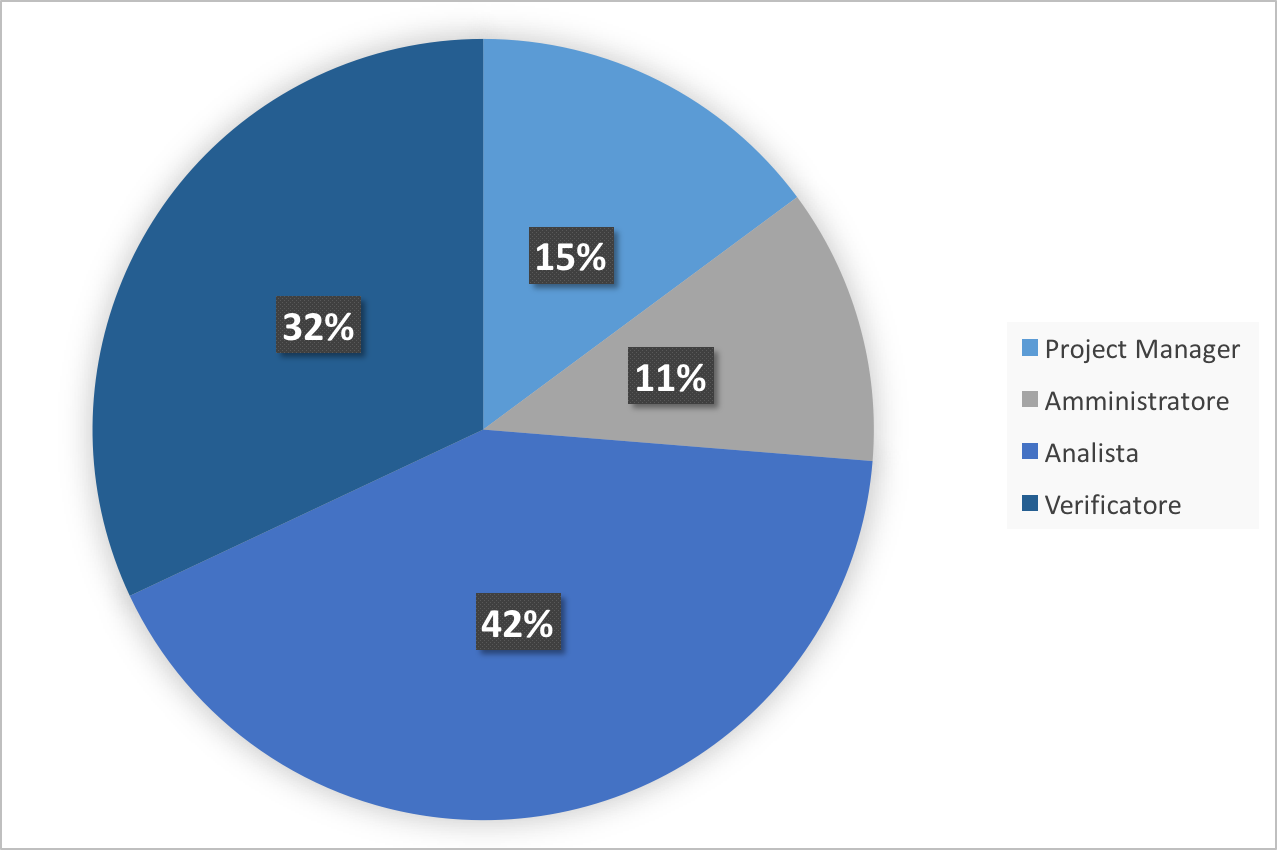
\includegraphics[scale=0.7]{Immagini/GraficiTorte/ARM.png}
	\caption{Ore per ruolo, \ARM}
\end{figure}

\newpage
\subsection{\ARD}
Le ore impiegate in questo periodo sono 39 e vengono ripartite in:

\begin{table}[h]
	\begin{center}
		\begin{tabular}{|c|c|}
			\hline
			\textbf{Ruolo}	& \textbf{Ore} \\
			\hline
			\Pm &	5\\
			\hline
			\Am	&	5\\
			\hline
			\An		&	18\\
			\hline
			\Ver	&	11\\
			\hline
		\end{tabular}
	\end{center}
	\caption{Ore per ruolo, \ARD}
\end{table}

\begin{figure}[H]
	\centering 
	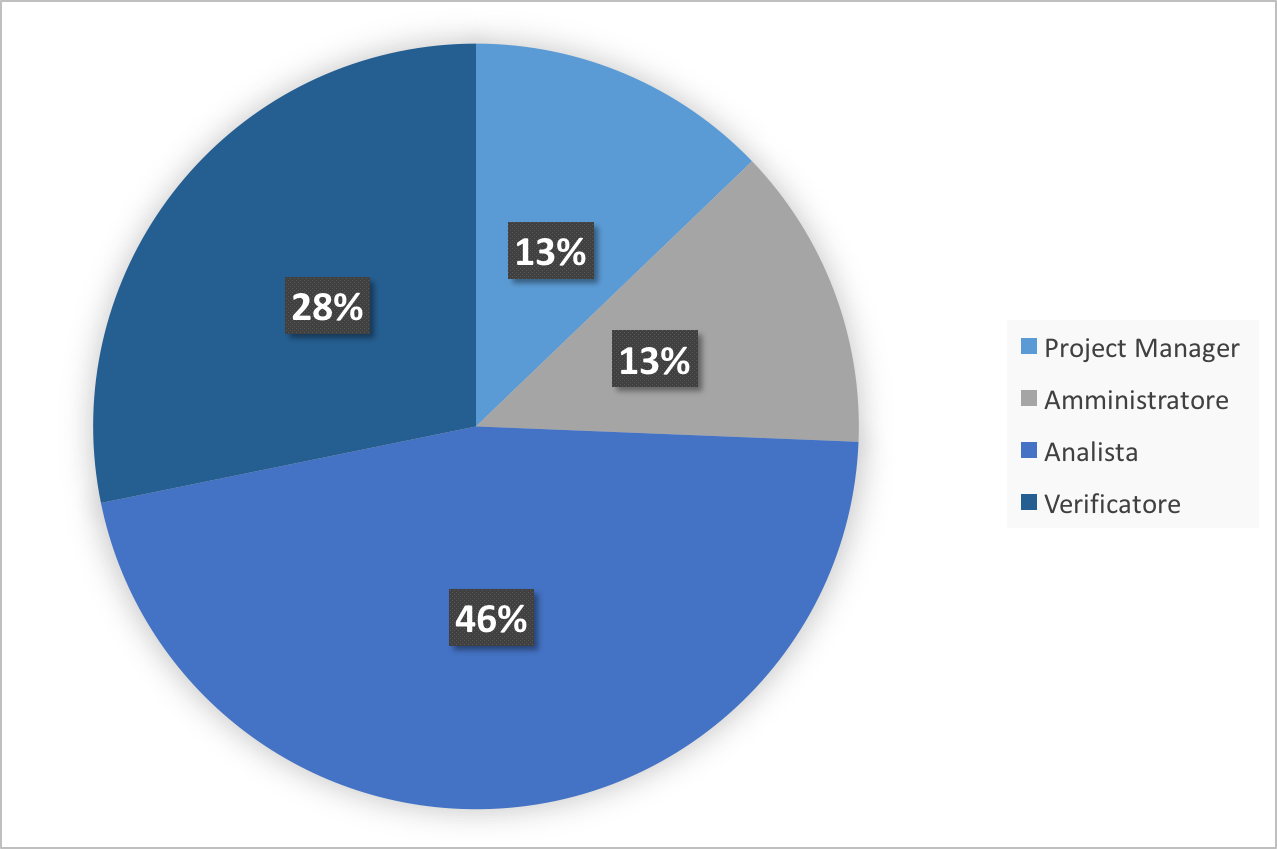
\includegraphics[scale=0.7]{Immagini/GraficiTorte/ARD.png}
	\caption{Ore per ruolo, \ARD}
\end{figure}
\newpage
\subsection{\PA}
Le ore totali impiegate in questo periodo sono 205 e vengono ripartite in:

\begin{table}[h]
	\begin{center}
		\begin{tabular}{|c|c|}
			\hline
			\textbf{Ruolo}	& \textbf{Ore} \\
			\hline
			\Pm &	6\\
			\hline
			\Am	&	8\\
			\hline
			\Prog		&	129\\
			\hline
			\Ver	&	62\\
			\hline
		\end{tabular}
	\end{center}
	\caption{Ore per ruolo, \PA}
\end{table}

\begin{figure}[H]
	\centering 
	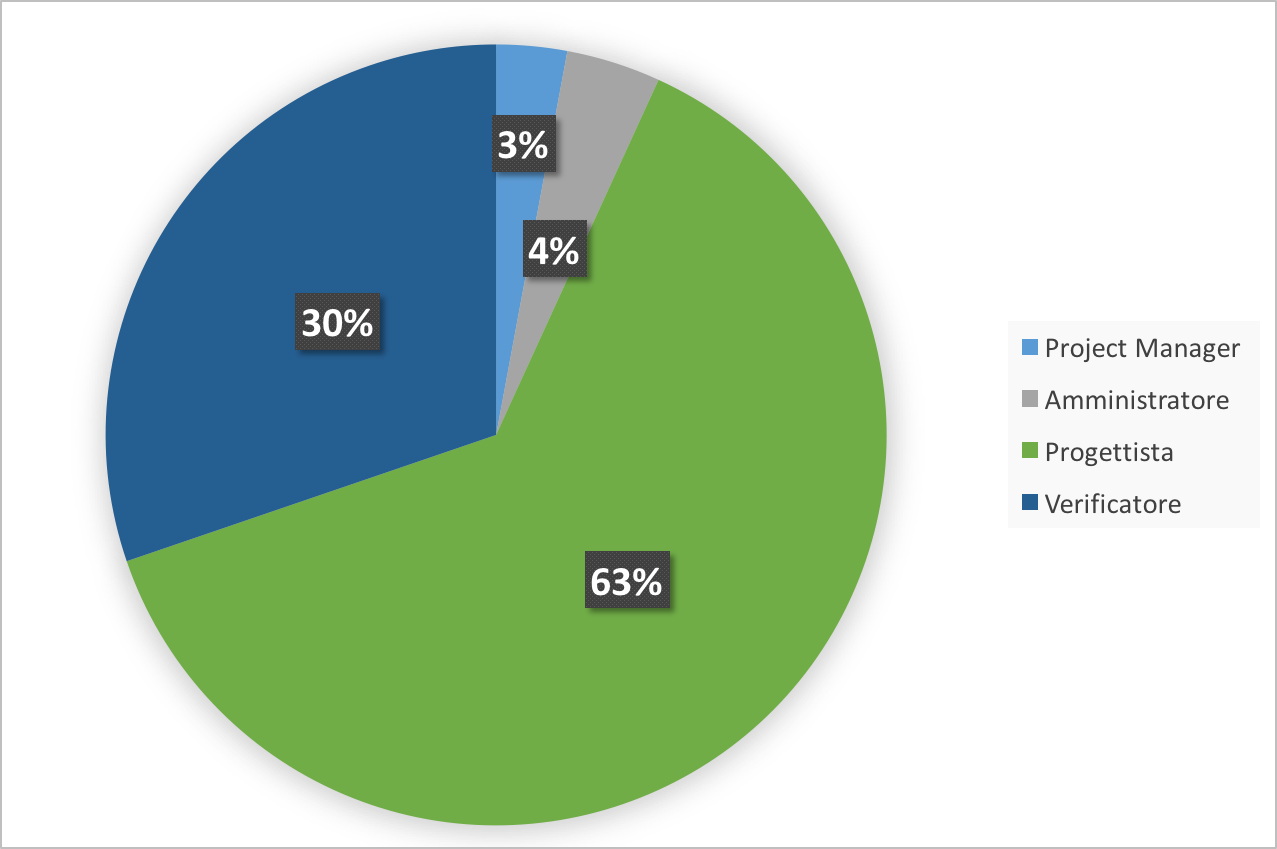
\includegraphics[scale=0.7]{Immagini/GraficiTorte/PA.png}
	\caption{Ore per ruolo, \PA}
\end{figure}
\newpage
\subsection{\PD}
Le ore impiegate in questo periodo sono 128 e vengono ripartite in:

\begin{table}[h]
	\begin{center}
		\begin{tabular}{|c|c|}
			\hline
			\textbf{Ruolo}	& \textbf{Ore} \\
			\hline
			\Pm &	7\\
			\hline
			\Am	&	7\\
			\hline
			\Prog		&	76\\
			\hline
			\Ver	&	38\\
			\hline
		\end{tabular}
	\end{center}
	\caption{Ore per ruolo, \PD}
\end{table}

\begin{figure}[H]
	\centering 
	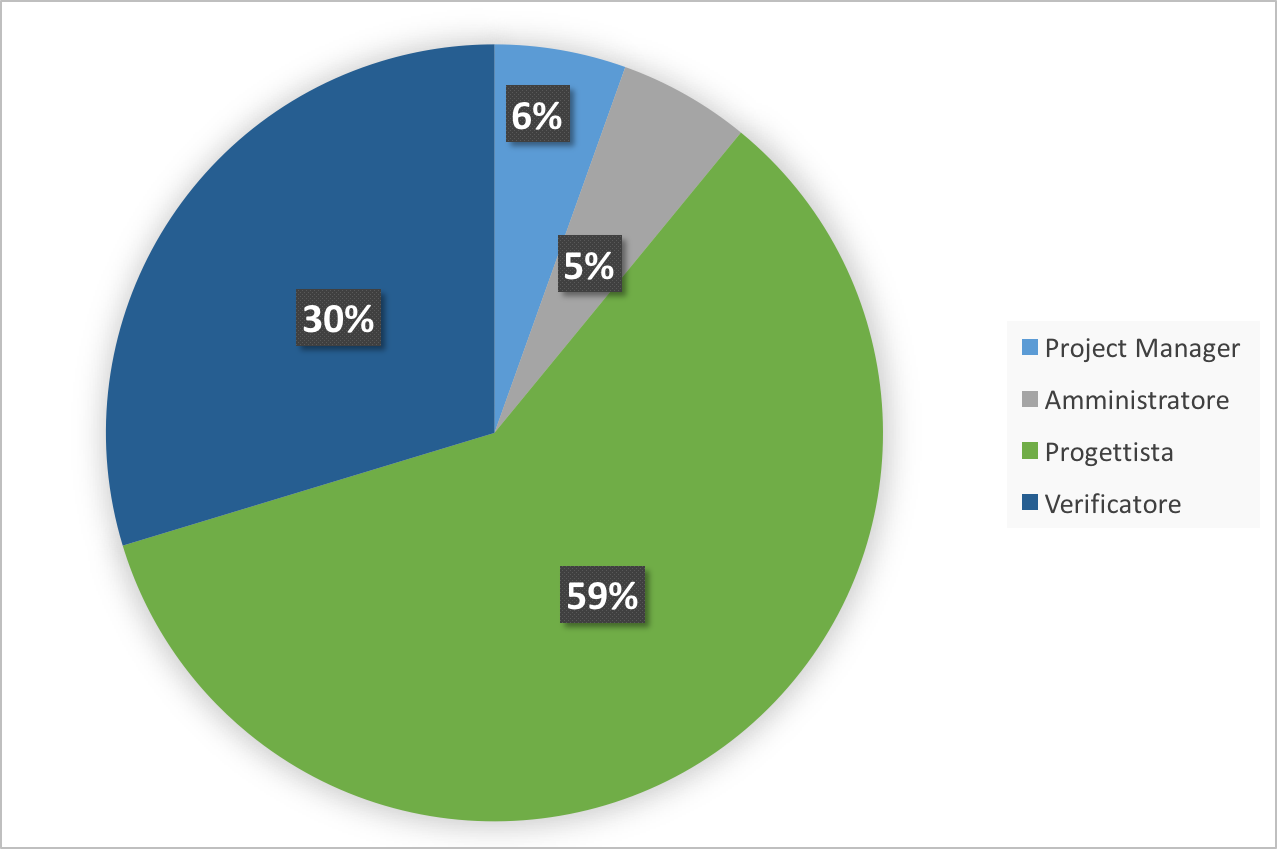
\includegraphics[scale=0.7]{Immagini/GraficiTorte/PD.png}
	\caption{Ore per ruolo, \PD}
\end{figure}
\newpage
\subsection{\COD}
Le ore impiegate in questo periodo sono 230 e vengono ripartite in:

\begin{table}[h]
	\begin{center}
		\begin{tabular}{|c|c|}
			\hline
			\textbf{Ruolo}	& \textbf{Ore} \\
			\hline
			\Pm &	11\\
			\hline
			\Am	&	6\\
			\hline
			\Prog		&	21\\
			\hline
			\Progr	&	132\\
			\hline
			\Ver	&	60\\
			\hline
		\end{tabular}
	\end{center}
	\caption{Ore per ruolo, \COD}
\end{table}

\begin{figure}[H]
	\centering 
	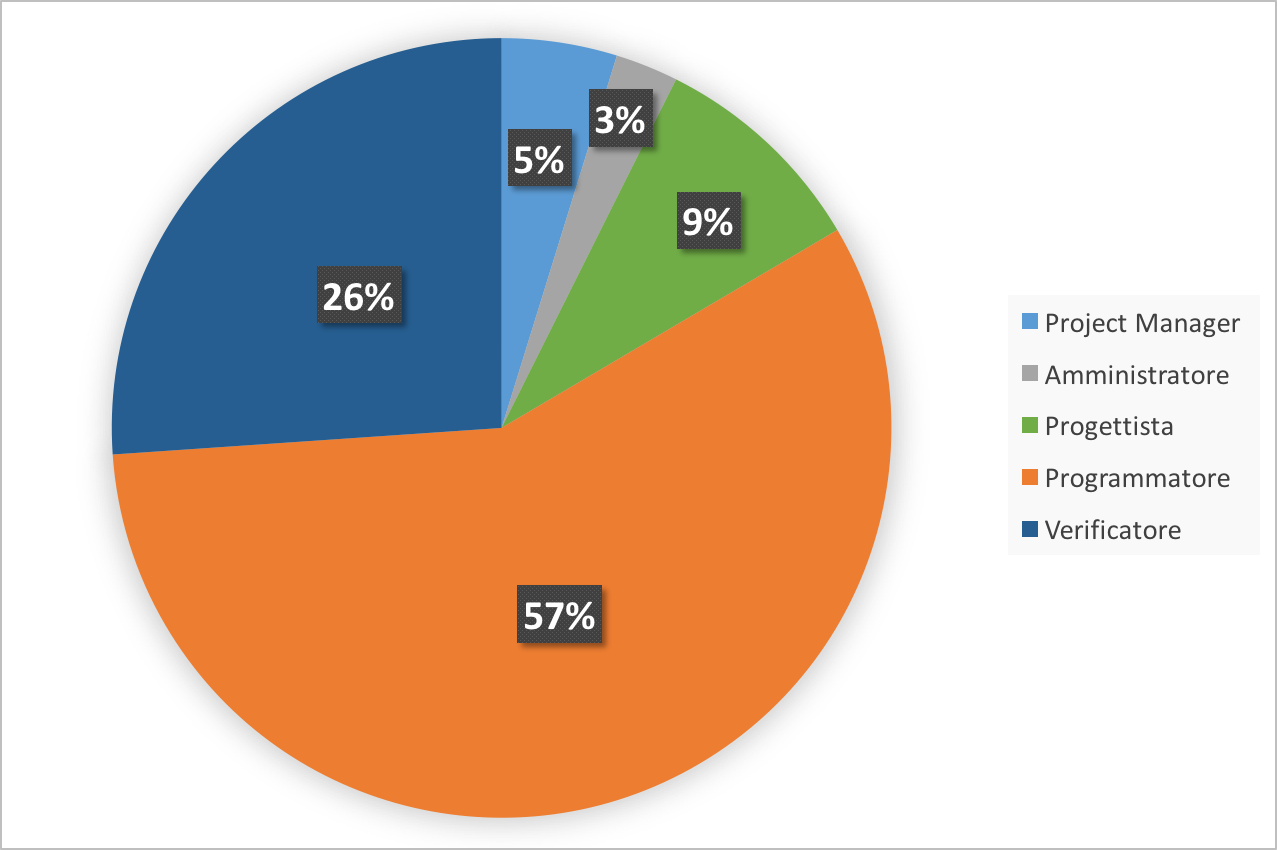
\includegraphics[scale=0.7]{Immagini/GraficiTorte/COD.png}
	\caption{Ore per ruolo, \COD}
\end{figure}
\newpage
\subsection{\VV}
Le ore totali in questo periodo sono 126 e vengono ripartite in:

\begin{table}[h]
	\begin{center}
		\begin{tabular}{|c|c|}
			\hline
			\textbf{Ruolo}	& \textbf{Ore} \\
			\hline
			\Pm &	12\\
			\hline
			\Am	&	8\\
			\hline
			\Prog		&	22\\
			\hline
			\Ver	&	84\\
			\hline
		\end{tabular}
	\end{center}
	\caption{Ore per ruolo, \VV}
\end{table}

\begin{figure}[H]
	\centering 
	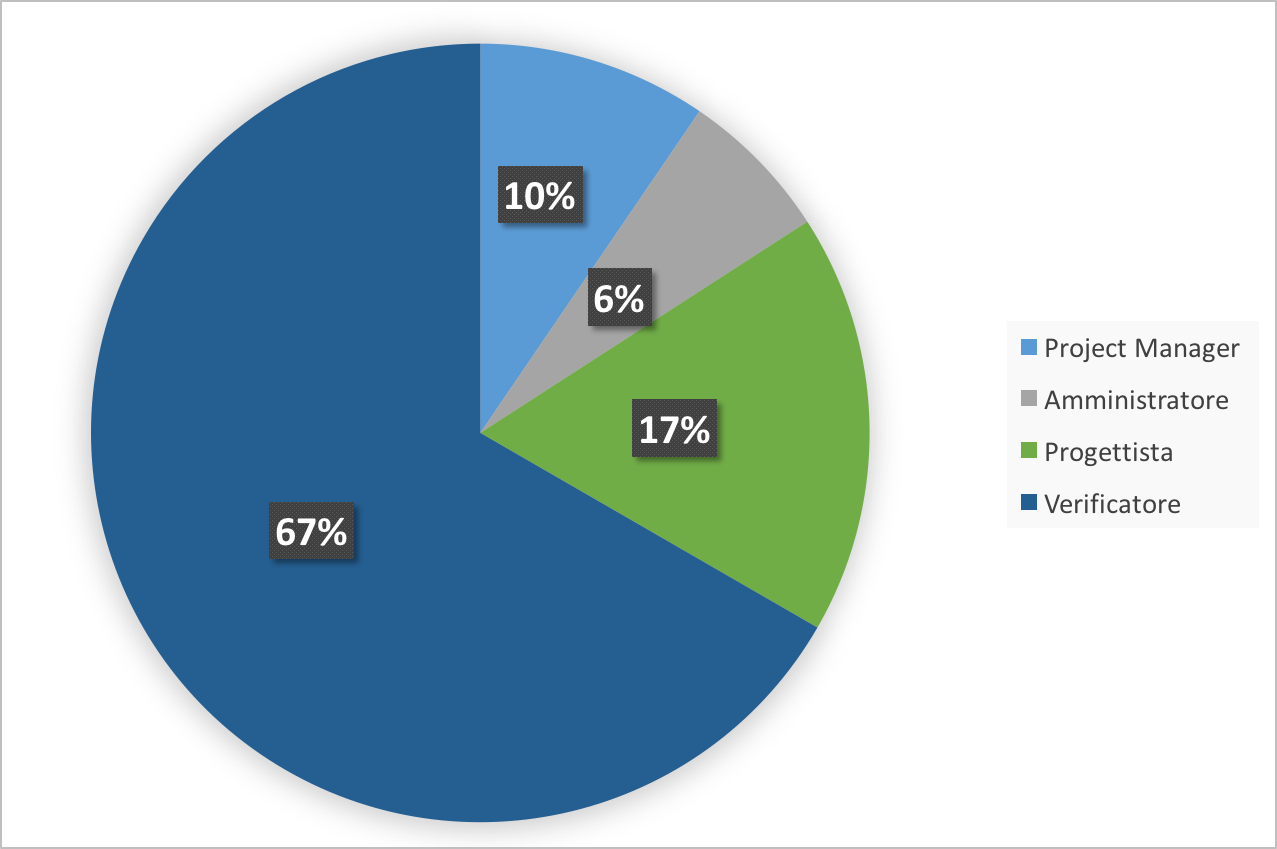
\includegraphics[scale=0.7]{Immagini/GraficiTorte/VV.png}
	\caption{Ore per ruolo, \VV}
\end{figure}
\newpage
\subsection{Quadro riassuntivo}
Le ore totali del progetto sono 903, di cui 728 remunerabili, così ripartite:

\begin{table}[h]
	\begin{center}
		\begin{tabular}{|c|c|c|}
			\hline
			\textbf{Ruolo}	& \textbf{Ore totali} & \textbf{Ore remunerabili} \\
			\hline
			\Pm &	67	&	41	\\
			\hline
			\Am	&	46	&	26	\\
			\hline
			\An		&	90	&	18	\\
			\hline
			\Prog		&	248	&	248	\\
			\hline
			\Progr	&	132	&	132	\\
			\hline
			\Ver	&	311	&	255	\\
			\hline
		\end{tabular}
	\end{center}
	\caption{Ore per ruolo, Quadro riassuntivo}
\end{table}

\begin{figure}[H]
	\centering 
	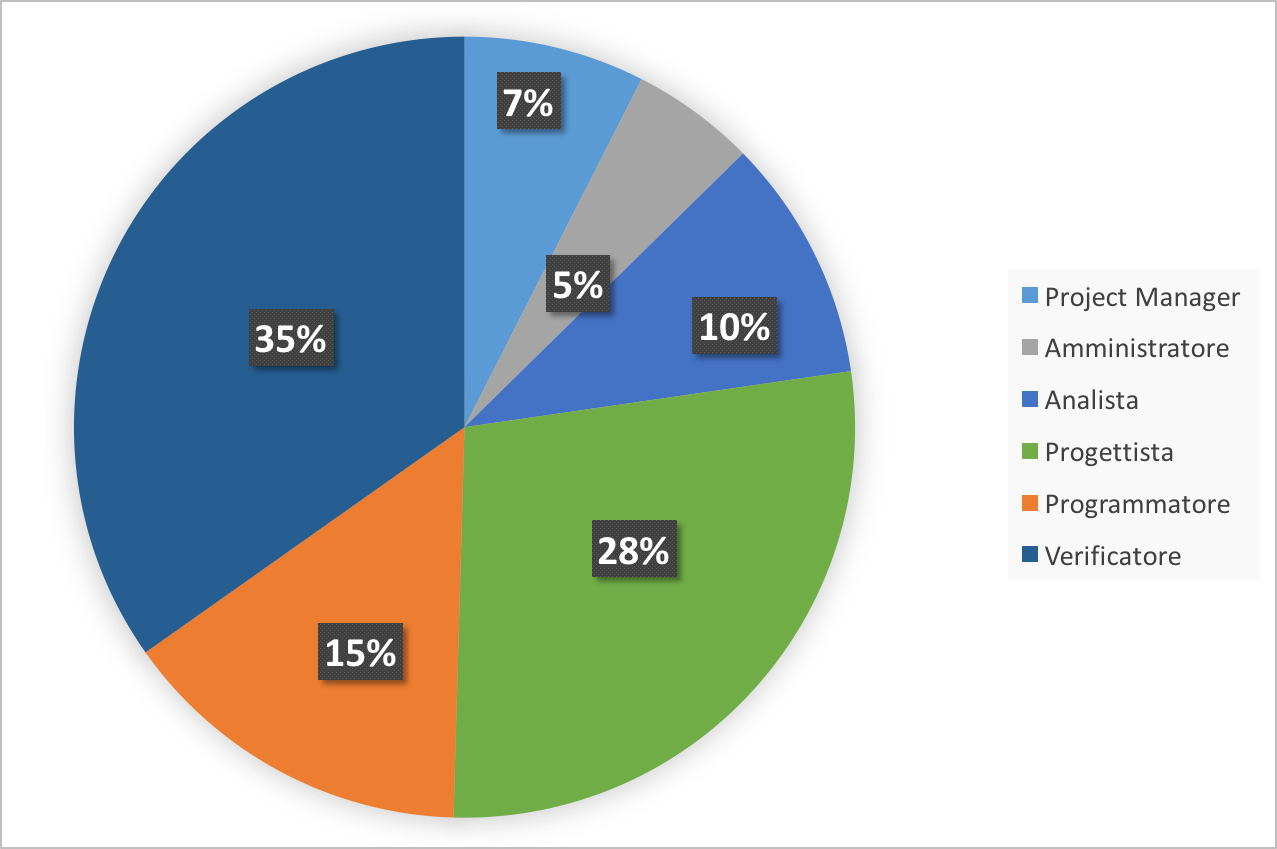
\includegraphics[scale=0.7]{Immagini/GraficiTorte/TOT.png}
	\caption{Ore totali per ruolo}
\end{figure}